\documentclass[12pt,a4paper]{article}

\usepackage{fancyhdr}
\usepackage{graphicx}
\usepackage{placeins}
\usepackage{adjustbox}


\begin{document}

\pagestyle{fancy}
\fancyhf{}
\chead{Short summary report}

\begin{table}[t]
\centering
\caption {rnaQUAST metrics for assembled transcripts. In each row the best values are indicated with \textbf{bold}. For the transcript metrics (rows 4, 5, 6, 9, 13, 25, 26, 27) we highlighted the best \textbf{relative} values i.e. divided by the total number of transcripts in the corresponding assembly.}
\begin{adjustbox}{width=1\textwidth}
\small
\begin{tabular}{|l*{11}{|r}|}
\hline
\textbf{METRICS/TRANSCRIPTS}                            & \textbf{Trinity}       & \textbf{Trans-ABySS}   & \textbf{Oases}         & \textbf{SOAPdenovo-Trans} & \textbf{IDBA-Tran}     & \textbf{Bridger}       & \textbf{BinPacker}     & \textbf{Shannon}       & \textbf{rnaSPAdes}     & \textbf{SPAdes}        \\ \hline\hline
\multicolumn{11}{l}{\bf DATABASE METRICS}                                                 \\ \hline
Genes                                                   & 12867                  & 12867                  & 12867                  & 12867                  & 12867                  & 12867                  & 12867                  & 12867                  & 12867                  & 12867                  \\
Avg. number of exons per isoform                        & 1.075                  & 1.075                  & 1.075                  & 1.075                  & 1.075                  & 1.075                  & 1.075                  & 1.075                  & 1.075                  & 1.075                  \\ \hline
\multicolumn{11}{l}{\bf BASIC TRANSCRIPTS METRICS}                                        \\ \hline
Transcripts                                             & 8970                   & 26356                  & 24818                  & 14927                  & 9408                   & 8413                   & 8324                   & 17225                  & 8297                   & 6821                   \\
Transcripts $>$ 500 bp                                  & 5578                   & 13304                  & 16371                  & 5424                   & 5711                   & 6159                   & \textbf{6485}          & 8567                   & 5614                   & 4858                   \\
Transcripts $>$ 1000 bp                                 & 3417                   & 7979                   & 9813                   & 2769                   & 2949                   & 4038                   & 4267                   & 4077                   & 3939                   & \textbf{3504}          \\ \hline
\multicolumn{11}{l}{\bf ALIGNMENT METRICS}                                                \\ \hline
Aligned                                                 & 8786                   & 25928                  & 24192                  & 14724                  & 9238                   & 8226                   & 8138                   & \textbf{17071}         & 8092                   & 6502                   \\
Uniquely aligned                                        & 5000                   & 14459                  & 14556                  & 7606                   & 5725                   & 4853                   & 4905                   & 8573                   & 4847                   & 3983                   \\
Multiply aligned                                        & 3565                   & 10667                  & 8399                   & 7073                   & 3484                   & 2796                   & 2610                   & 7282                   & 2961                   & 2393                   \\
Unaligned                                               & 184                    & 428                    & 626                    & 203                    & 170                    & 187                    & 186                    & \textbf{154}           & 205                    & 319                    \\ \hline
\multicolumn{11}{l}{\bf ALIGNMENT METRICS FOR NON-MISASSEMBLED TRANSCRIPTS}               \\ \hline
Avg. aligned fraction                                   & 0.994                  & 0.988                  & 0.986                  & \textbf{0.997}         & 0.996                  & 0.987                  & 0.985                  & 0.993                  & 0.988                  & 0.99                   \\
Avg. alignment length                                   & 969.327                & 773.584                & 941.6                  & 567.169                & 922.096                & 1131.326               & 1189.552               & 678.947                & 1171.714               & \textbf{1279.411}      \\
Avg. mismatches per transcript                          & 1.819                  & 1.288                  & 2.121                  & \textbf{0.569}         & 0.807                  & 1.996                  & 2.283                  & 0.999                  & 1.959                  & 1.799                  \\ \hline
\multicolumn{11}{l}{\bf ALIGNMENT METRICS FOR MISASSEMBLED (CHIMERIC) TRANSCRIPTS}          \\ \hline
Misassemblies                                           & 72                     & 449                    & 613                    & \textbf{9}             & 8                      & 236                    & 259                    & 362                    & 82                     & 60                     \\ \hline
\multicolumn{11}{l}{\bf ASSEMBLY COMPLETENESS (SENSITIVITY)}                              \\ \hline
Database coverage                                       & 0.511                  & \textbf{0.653}         & 0.604                  & 0.564                  & 0.527                  & 0.476                  & 0.47                   & 0.541                  & 0.508                  & 0.485                  \\
50\%-assembled genes                                    & 5302                   & \textbf{6734}          & 6425                   & 5362                   & 5380                   & 5136                   & 5162                   & 5475                   & 5413                   & 5266                   \\
95\%-assembled genes                                    & 4146                   & \textbf{5214}          & 4808                   & 3290                   & 3238                   & 4005                   & 4033                   & 3736                   & 4533                   & 4437                   \\
50\%-covered genes                                      & 6011                   & \textbf{7833}          & 7237                   & 6742                   & 6229                   & 5581                   & 5556                   & 6884                   & 5819                   & 5529                   \\
95\%-covered genes                                      & 4585                   & \textbf{5884}          & 5450                   & 4522                   & 4003                   & 4322                   & 4343                   & 4562                   & 4783                   & 4542                   \\
50\%-assembled isoforms                                 & 5302                   & \textbf{6734}          & 6425                   & 5362                   & 5380                   & 5136                   & 5162                   & 5475                   & 5413                   & 5266                   \\
95\%-assembled isoforms                                 & 4146                   & \textbf{5214}          & 4808                   & 3290                   & 3238                   & 4005                   & 4033                   & 3736                   & 4533                   & 4437                   \\
50\%-covered isoforms                                   & 6011                   & \textbf{7833}          & 7237                   & 6742                   & 6229                   & 5581                   & 5556                   & 6884                   & 5819                   & 5529                   \\
95\%-covered isoforms                                   & 4585                   & \textbf{5884}          & 5450                   & 4522                   & 4003                   & 4322                   & 4343                   & 4562                   & 4783                   & 4542                   \\
Mean isoform coverage                                   & 0.817                  & 0.832                  & 0.819                  & 0.756                  & 0.771                  & 0.809                  & 0.82                   & 0.771                  & 0.849                  & \textbf{0.852}         \\
Mean isoform assembly                                   & 0.746                  & 0.748                  & 0.749                  & 0.629                  & 0.687                  & 0.76                   & 0.776                  & 0.66                   & 0.806                  & \textbf{0.822}         \\ \hline
\multicolumn{11}{l}{\bf ASSEMBLY SPECIFICITY}                                             \\ \hline
50\%-matched                                            & 7488                   & 20937                  & 19840                  & 12185                  & \textbf{7998}          & 6537                   & 6370                   & 14640                  & 6225                   & 5246                   \\
95\%-matched                                            & 3529                   & 10745                  & 9568                   & 7596                   & 3595                   & 2587                   & 2313                   & \textbf{8873}          & 2206                   & 1793                   \\
Unannotated                                             & 591                    & 2559                   & 1653                   & 1706                   & 574                    & 502                    & 495                    & \textbf{604}           & 884                    & 568                    \\
Mean fraction of transcript matched                     & 0.799                  & 0.765                  & 0.789                  & 0.775                  & 0.786                  & 0.771                  & 0.761                  & \textbf{0.867}         & 0.708                  & 0.732                  \\ \hline
\end{tabular}
\end{adjustbox}
\end{table}

\FloatBarrier
\clearpage
\lfoot{generated by rnaQUAST}

\begin{figure}[t]
\centering
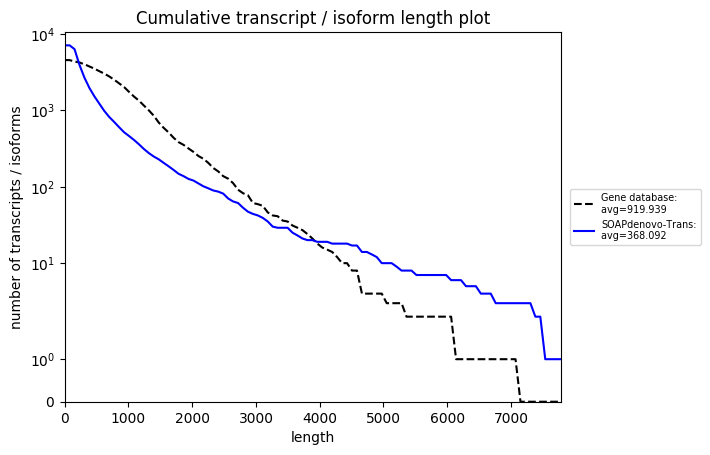
\includegraphics[width = \linewidth]{/mnt/dessertlocal/projects/transcriptome_assembly/review/evaluation/rna-quast/cal/comparison_output/transcript_length.png}
\caption{Plot showing cumulative transcript length distribution. Each point represents the number of transcripts in the assembly with the corresponding length or longer; black dashed line corresponds to the database isoforms; the plot is given in logarithmic scale.}
\end{figure}
\FloatBarrier
\clearpage


\begin{figure}[t]
\centering
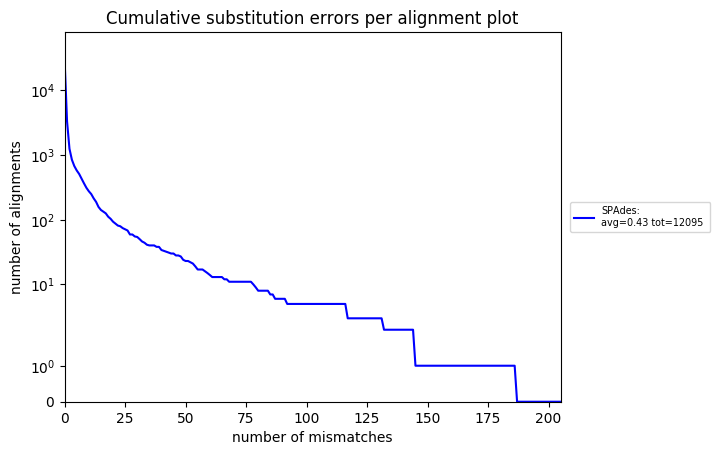
\includegraphics[width = \linewidth]{/mnt/dessertlocal/projects/transcriptome_assembly/review/evaluation/rna-quast/cal/comparison_output/mismatch_rate.png}
\caption{Plot showing cumulative substitution errors per alignment distribution. Each point represents the number of alignments with the corresponding number of mismatches or greater; the plot is given in logarithmic scale.}
\end{figure}
\FloatBarrier
\clearpage


\begin{figure}[t]
\centering
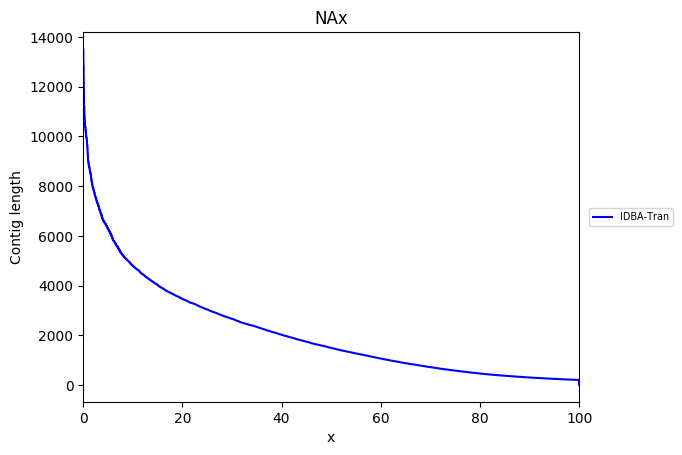
\includegraphics[width = \linewidth]{/mnt/dessertlocal/projects/transcriptome_assembly/review/evaluation/rna-quast/cal/comparison_output/NAx.png}
\caption{Nx plot for transcripts. Nx is a maximal number $N$, such that the total length of all transcripts longer than $N$ bp is at least $x\%$ of the total length of all transcripts.}
\end{figure}
\FloatBarrier
\clearpage


\begin{figure}[t]
\centering
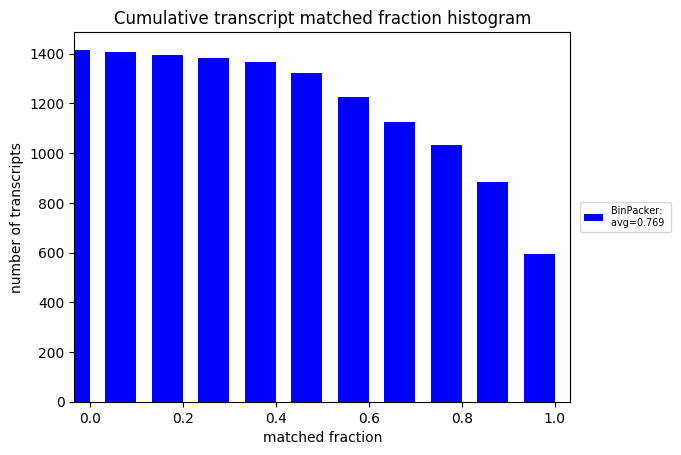
\includegraphics[width = \linewidth]{/mnt/dessertlocal/projects/transcriptome_assembly/review/evaluation/rna-quast/cal/comparison_output/x-matched.png}
\caption{Plot showing cumulative transcript match histogram. Each bar represents the number of transcripts with matched fraction equal to or greater than the value on $x$ axis; transcript matched fraction is calculated as the number of its bases covering an isoform divided by the transcript length.}
\end{figure}
\FloatBarrier
\clearpage


\begin{figure}[t]
\centering
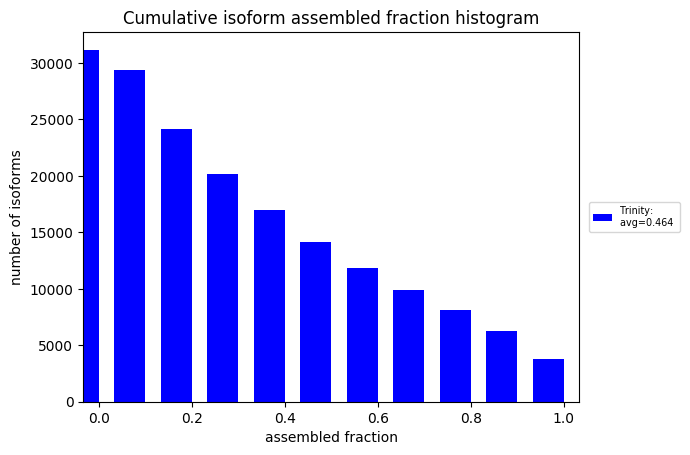
\includegraphics[width = \linewidth]{/mnt/dessertlocal/projects/transcriptome_assembly/review/evaluation/rna-quast/cal/comparison_output/x-assembled.png}
\caption{Plot showing cumulative isoform assembly histogram. Each bar represents the number of isoforms with assembled fraction equal to or greater than the value on $x$ axis; isoform assembled fraction is calculated as the maximum number of captured by single assembled transcript bases divided by the total isoform length.}
\end{figure}
\FloatBarrier
\clearpage


\begin{figure}[t]
\centering
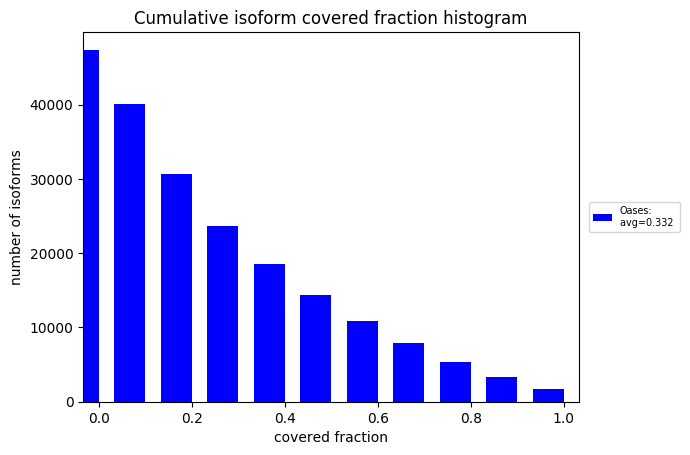
\includegraphics[width = \linewidth]{/mnt/dessertlocal/projects/transcriptome_assembly/review/evaluation/rna-quast/cal/comparison_output/x-covered.png}
\caption{Plot showing cumulative isoform coverage histogram. Each bar represents the number of isoforms with covered fraction equal to or greater than the value on $x$ axis; isoform covered fraction is calculated as the number of covered bases (by all transcripts in the assembly) divided by the total isoform length.}
\end{figure}
\FloatBarrier
\clearpage


\end{document}
